\documentclass{article}
\usepackage{graphicx} % Required for inserting images
\usepackage{float}
\usepackage{booktabs}
\title{Lesson 2 Homework - Calculus}
\author{William Wang}
\date{August 2026}

\begin{document}

\maketitle

\section{}
\subsection{}
Let 
\[f(x) = \frac{x-3}{x-4}\]
Then if we let \(c = 1\), \(x-3 \neq 0\) and \(x-4 \neq 0\). We have 
\[\lim_{x \to 1} f(x) = \frac{\lim_{x\to1}x-3}{\lim_{x\to1}x-4} = \frac{2}{3}\]
Then if we let \(c = 3\), \(x-3 = 0\) and \(x-4\neq 0\). We have 
\[\lim_{x\to3} f(x) = \frac{\lim{x\to3}x-3}{\lim_{x\to3}x-4} = 0\]
\subsection{}
\begin{figure}[H]
    \centering
    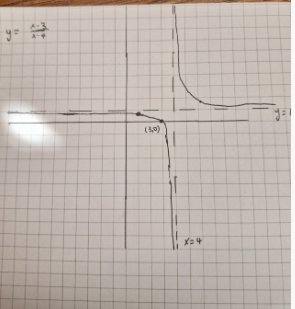
\includegraphics[width=0.5\linewidth]{image4.png}
\end{figure}
\subsection{}
Let 
\[f(x) = \frac{x-3}{x-4}\]  
Then if \(x = c = 4\), \(x-4 = 0\). Then we have 
\[\lim_{x\to4} f(x)\]
\begin{table}[ht]
\centering
\begin{tabular}{cc}
\toprule
$x$ & $f(x)$ \\
\midrule
$4.1$    & $11$ \\
$4.01$   & $101$ \\
$4.001$  & $1001$ \\
$4.0001$ & $10001$ \\

$3.9$& $-9$ \\
$3.99$   & $-99$ \\
$3.999$    & $-999$ \\
$3.9999$     & $-9999$ \\
\bottomrule
\end{tabular}
\end{table}
This shows that if we approach \(x \to 4^-\) it approaches negative infinity and if we approach \(x \to 4^+\) it approaches positive infinity. Since the limit approaches infinity, the limit is undefined. 
\subsection{}
If \(p(c) \neq 0\) and \(q(c) = 0\) then near \(x = c\) the denominator is very close to $0$ while the numerator stays close to some nonzero number. Dividing a nonzero number by one that gets closer and closer to $0$ means that the results produce values with arbitrarily large magnitude.This means
\[|f(x)| \to \infty\]
This means that the limit is always undefined in this case. 
\subsection{}
\subsubsection{}
We have 
\[f_1(x) = \frac{x^2-3x+2}{x^2+2x-3} = \frac{(x-2)(x-1)}{(x+3)(x-1)}\]
We can cancel the \(x-1\) the functions are the exact same except for the hole at \(x = 1\). Since we are taking the limit as \(x\to 1\) we are not interested in what happens at \(x=1\). Hence we can cancel. 
\[\lim_{x \to 1} f_1(x) = \lim_{x\to 1} \frac{x-2}{x+3} = \frac{-1}{4}\]
\begin{figure}[H]
    \centering
    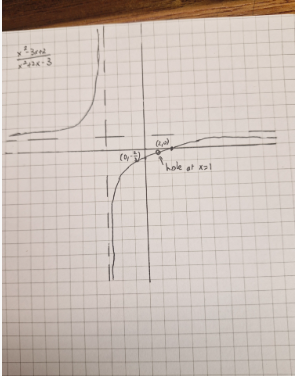
\includegraphics[width=0.5\linewidth]{image3.png}
\end{figure}
As we can see from the graph, there is a hole at \(x=1\). However, the limit is still defined since we can see that the function approached that point from either side. 

\subsubsection{}
We have 
\[f_2(x) = \frac{x-1}{x^2-2x+1} = \frac{x-1}{(x-1)^2}\]
We can cancel the \(x-1\) the functions are the exact same except for the hole at \(x = 1\). Since we are taking the limit as \(x\to 1\) we are not interested in what happens at \(x=1\). Hence we can cancel. 
\[\lim_{x\to1} f_2(x) = \lim_{x\to1} \frac{1}{x-1}\]
This becomes case 3 which we know is undefined. 
\begin{figure}[H]
    \centering
    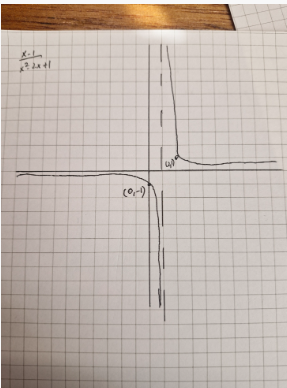
\includegraphics[width=0.5\linewidth]{image2.png}
\end{figure}
From the graph, we can clearly see that \(x = 1\) is an asymptote of the function, hence the limit is undefined as the function never approaches that point. 
\subsubsection{}
We have 
\[f_3(x) = \frac{x^2-2x+1}{x-1} = \frac{(x-1)^2}{x-1}\]
We can cancel the \(x-1\) the functions are the exact same except for the hole at \(x = 1\). Since we are taking the limit as \(x\to 1\) we are not interested in what happens at \(x=1\). Hence we can cancel. 
\[\lim_{x \to 1} f_3(x) = \lim_{x\to1} x-1 = 0\]
\begin{figure}[H]
    \centering
    
\includegraphics[width=0.5\linewidth]{image.png}
\end{figure}
Similar to the first function, there is a hole at \(x = 1\) but the limit is still defined since the limit is just the behavior of the function as it approaches \(x = 1\) which we have computed as $0$
\subsection{}
We can't make assumptions about the behavior of the limit since it could have an actual value if but the limit could also be undefined so we can't draw any assumption about it. For example \(f_1(x)\) has a valid limit as \(x \to 1\) but \(f_2(x)\) doesn't. We do know that the function is undefined at \(c\). 
\subsection{}
Case 1: \(L \neq 0\) and \(M \neq 0\), the limit exists as \(x \to c\). Case 2: \(L = 0\) and \(M \neq 0\), the limit is always \(0\) as \(x \to c\). Case 3: \(L \neq 0\) and \(M = 0\), the limit doesn't exist and there will always be a vertical asymptote at \(x=c\) . Case 4: \(L = 0\) and \(M = 0\), can't draw any assumptions, need to further simplify but we do know that the function is undefined at \(x=c\) which means that there is either a hole or a vertical asymptote. 
\end{document}
